\documentclass[12pt, a4paper]{article}

% --- KHAI BÁO CÁC THƯ VIỆN CẦN THIẾT ---
\usepackage[utf8]{vietnam} 
%(Trái/Phải: 1.3cm, Trên/Dưới: 1.5cm)
\usepackage[left=1.3cm, right=1.3cm, top=1.5cm, bottom=1.5cm]{geometry}
%Phông chữ Times New Roman
\usepackage{mathptmx}
%Cấu hình khoảng cách dòng 1 line spacing
\usepackage{setspace}
\singlespacing

%Toán số học, ký hiệu toán học
\usepackage{amsmath}

%Graph, biểu đồ
\usepackage{pgfplots}
\pgfplotsset{compat=1.18}

\usepackage{graphicx}
\usepackage{authblk} 
\usepackage{titlesec}
\usepackage{cite}
\usepackage{subcaption}

% --- THƯ VIỆN VẼ SƠ ĐỒ ---
\usepackage{tikz}
\usetikzlibrary{shapes.geometric, positioning, arrows.meta}

% --- TRÌNH BÀY CODE (PYTHON) ---
\usepackage{minted}

% --- URL ---
\usepackage[colorlinks=true, urlcolor=black, linkcolor=black, citecolor=blue]{hyperref}
\graphicspath{{../}}

% --- CẤU HÌNH TIÊU ĐỀ BÀI BÁO (Dành cho trang 2) ---
\titleformat{\section}{\normalfont\Large\bfseries}{\thesection}{1em}{}
\title{\textbf{Dự đoán thời gian ùn tắc giao thông}}

% --- CẤU HÌNH KÍCH THƯỚC CHỮ TÁC GIẢ ---
\renewcommand\Authfont{\small}          
\renewcommand\Affilfont{\itshape\small} 
\renewcommand*{\Authand}{, }            
\renewcommand*{\Authands}{, }           

\author{Nguyễn Lê Phúc Thịnh}
\author{Nguyễn Tuấn Thịnh}

\affil{Khoa Điện - Điện tử, Trường Đại học Công nghệ Kỹ thuật TP.HCM}
\affil{Giảng viên hướng dẫn: TS. Phan Học}

\date{} 

\begin{document}

% =======================================================
% TRANG 1: TRANG BÌA
% =======================================================
\begin{titlepage}
    \begin{center}
        \large \textbf{BỘ GIÁO DỤC VÀ ĐÀO TẠO} \\
        \large \textbf{TRƯỜNG ĐẠI HỌC CÔNG NGHỆ KỸ THUẬT TP.HCM} \\
        \large \textbf{KHOA ĐIỆN - ĐIỆN TỬ} \\
        \vspace{1.5cm} 
        
        
\includegraphics[width=4cm]{UTE_logo.png} 
        
        \vspace{1.5cm}
        \textbf{\huge BÁO CÁO CUỐI KỲ} \\
        \vspace{0.5cm}
        \large MÔN HỌC: CẤU TRÚC RỜI RẠC \\
        \vspace{1cm}
        \textbf{\Large DỰ ĐOÁN THỜI GIAN ÙN TẮC GIAO THÔNG} \\
        \vspace{2.5cm}
    \end{center}

    \begin{flushleft}
        \large
        \begin{tabular}{ll}
            \textbf{Giảng viên hướng dẫn:} & TS. Phan Học \\
            \textbf{Mã lớp học phần:} & [UTE] 261DSCC235864\_03 \\
            \\
            \textbf{Danh sách sinh viên thực hiện:} & \\
            1. Nguyễn Lê Phúc Thịnh & 25139047 \\
            2. Nguyễn Tuấn Thịnh & 25139048 \\
        \end{tabular}
    \end{flushleft}

    \vfill 
    
    \begin{center}
        \large TP. Hồ Chí Minh, tháng 10 năm 2026
    \end{center}
\end{titlepage}

% =======================================================
% TRANG 2: BẮT ĐẦU NỘI DUNG BÀI BÁO
% =======================================================
% --- MỤC LỤC ---
\tableofcontents
\newpage
% ---------------

\setcounter{page}{1} 
% \maketitle



% \begin{abstract}
% ... Ghi gì đó ở đây ...
% \end{abstract}

\section{Phát biểu bài toán}

    \subsection{Mục tiêu và phạm vi}
    Dự án nghiên cứu khả năng sử dụng ảnh camera tại khu vực Ngã Tư Hàng Xanh để theo dõi mức hiện diện của phương tiện và ước lượng thời gian đến một trạng thái đông xe. Hệ thống chuyển ảnh thành số đếm theo loại phương tiện, xây dựng chuỗi thời gian, dự báo diễn biến trong một giờ tiếp theo và trình bày kết quả trên ứng dụng desktop.

    Phiên bản đã triển khai giải quyết một bài toán cụ thể: dự báo chỉ số WTI(Weighted Traffic Index - Chỉ số tải trọng giao thông) trung bình từng phút trong 60 phút tiếp theo, sau đó xác định thời điểm bắt đầu cửa sổ vượt ngưỡng WTI thử nghiệm. Đây là hệ thống nguyên mẫu phục vụ nghiên cứu. Tập dữ liệu chưa có nhãn ùn tắc độc lập, tốc độ dòng xe hoặc thời gian hành trình để xác nhận trạng thái ùn tắc ngoài thực tế.

    \begin{figure}[htbp]
        \centering
        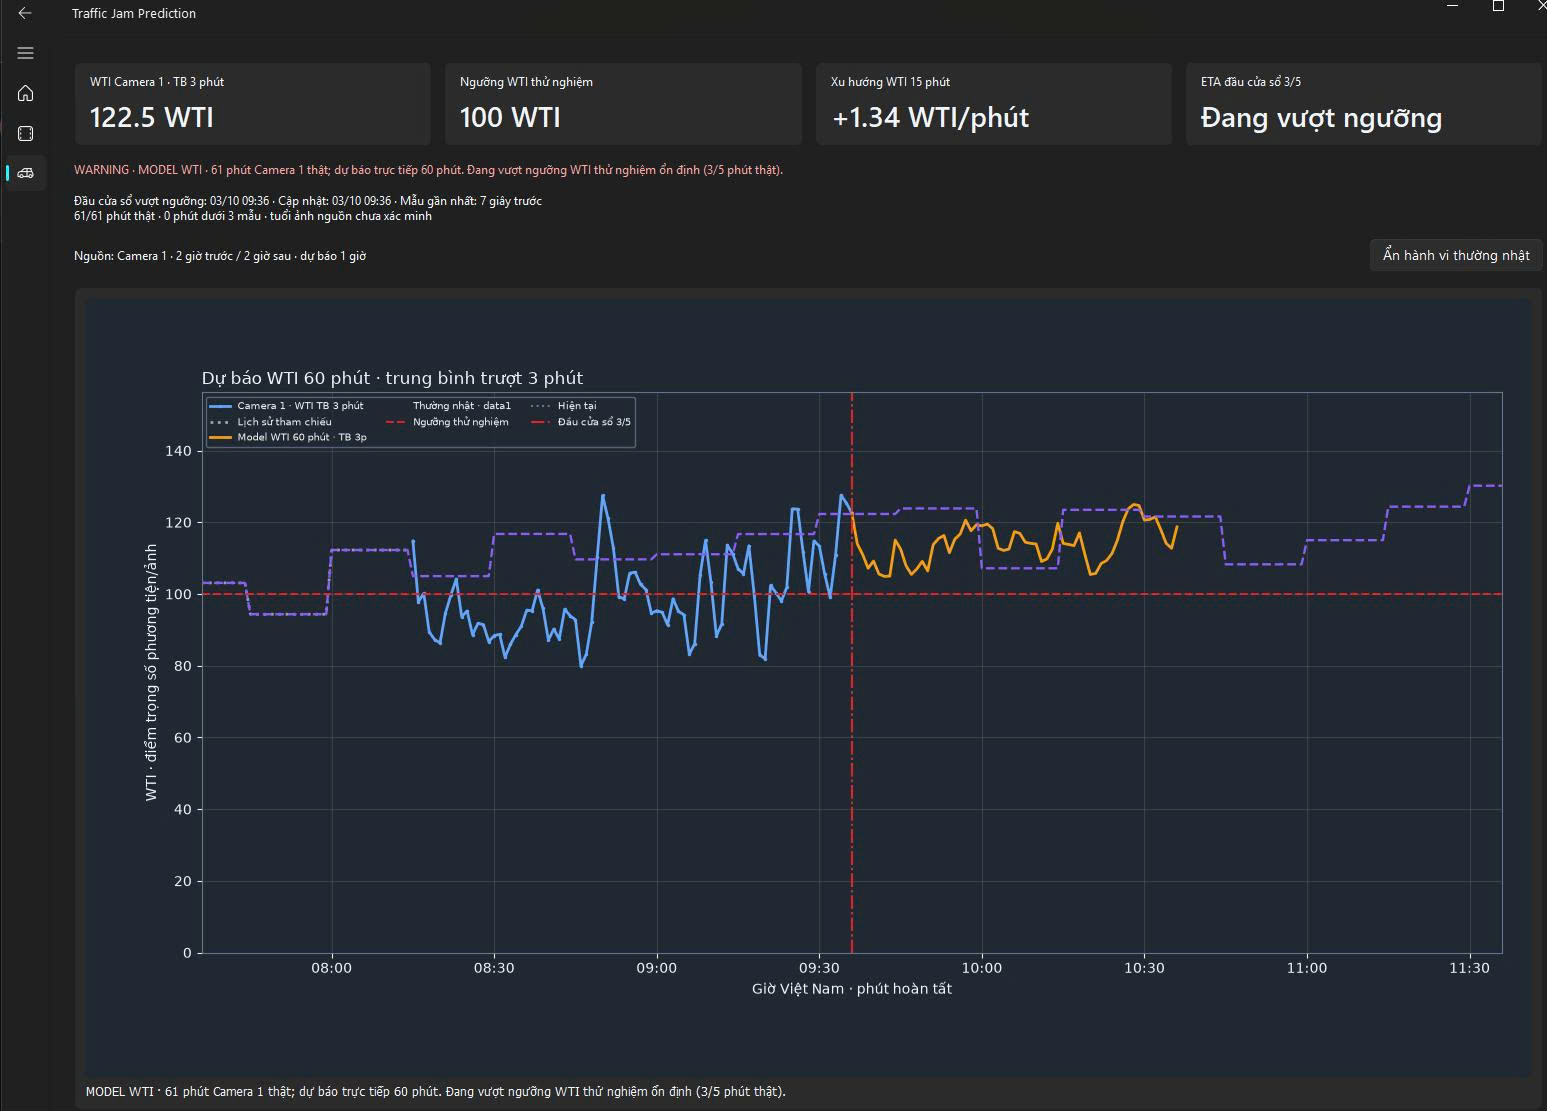
\includegraphics[width=0.9\textwidth]{runs/run.jpg} 
        \caption{Ảnh hiển thị chế độ MODEL WTI với 61 phút quan sát thật, WTI trung bình trượt 122,5 và trạng thái đang vượt ngưỡng. Trục hiển thị hai giờ trước và hai giờ sau hiện tại; phần dự báo chỉ dài 60 phút.}
    \end{figure}

    Kết quả đánh giá lưu trong dự án cho thấy mô hình đạt MAE (Maximum Average Error - Sai số tuyệt đối trung bình) là 14,12 WTI, thấp hơn khoảng 23,9\% so với cách giữ nguyên giá trị hiện tại. Tuy nhiên, lợi thế so với tham chiếu cùng giờ chỉ khoảng 4,0\%; tham chiếu này còn tốt hơn về một số chỉ số cảnh báo. Đóng góp rõ nhất của dự án là xây dựng được chuỗi xử lý từ ảnh đến dự báo có thể theo dõi và đánh giá, đồng thời làm rõ những giới hạn của phép đo dựa trên số xe trong ảnh.

    

    \subsection{Đầu vào và đầu ra}
    
    \begin{table}[htbp]
        \centering
        \caption{Đầu vào và đầu ra của hệ thống}
        \vspace{0.2cm}
        \begin{tabular}{|p{3cm}|p{6cm}|p{6cm}|}
            \hline
            \textbf{Cấp xử lý} & \textbf{Đầu vào} & \textbf{Đầu ra} \\
            \hline
            Thu ảnh & Snapshot camera từ nguồn giao thông công cộng TP.HCM, tải bằng HTTP & Ảnh màu BGR được OpenCV giải mã \\
            \hline
            Nhận diện & Ảnh và trọng số \texttt{yolo26x.pt} & Khung nhận diện; số lượng người, ô tô, xe máy, xe buýt, xe tải \\
            \hline
            Xây dựng dữ liệu & Timestamp, số xe và WTI trên từng ảnh & CSV gồm 9 cột; dữ liệu tổng hợp theo phút \\
            \hline
            Dự báo học máy & 61 đặc trưng từ phút hiện tại và tối đa 60 phút quá khứ & 60 giá trị WTI tương ứng $t+1$ đến $t+60$ \\
            \hline
            Cảnh báo & Đường dự báo được làm mượt và ngưỡng 100 WTI & ETA đến đầu cửa sổ vượt ngưỡng; trạng thái cảnh báo và chất lượng dữ liệu \\
            \hline
            Vận hành & Quan sát thật, tham chiếu và dự báo & Dashboard PyQt5, nhật ký mẫu và dự báo trong SQLite \\
            \hline
        \end{tabular}
    \end{table}

    Đại lượng trung tâm được định nghĩa trực tiếp trong mã nhận diện:
    \[ WTI = 4 \times \text{car} + 1 \times \text{motorbike} + 7 \times \text{bus} + 6 \times \text{truck} \]

    Trong đó, \textit{total} là tổng bốn loại xe; \textit{person} không tham gia \textit{total} hoặc \textit{WTI}. WTI là điểm số có trọng số trên một ảnh. Đơn vị này không tương đương xe/phút, xe/km hay xác suất ùn tắc. Các trọng số là quy ước của dự án; thư mục chưa cung cấp một thực nghiệm hiệu chuẩn chúng với mức chiếm dụng đường hoặc mức chậm trễ giao thông.

    Gọi $y(t)$ là WTI\_mean tại phút hoàn tất $t$, mô hình học ánh xạ từ $X(t)$ sang vector $[y(t+1), \dots, y(t+60)]$. ETA được suy ra từ vector dự báo.

    \subsection{Từ đề xuất ban đầu đến hệ thống hiện tại}
    Tài liệu Word là báo cáo đề xuất, trong đó có các phương án và công việc dự kiến. Đối chiếu với mã nguồn cho thấy những thay đổi sau:

    \begin{table}[htbp]
        \centering
        \caption{Đối chiếu đề xuất ban đầu và hệ thống hiện tại}
        \vspace{0.2cm}
        \begin{tabular}{|p{3.5cm}|p{5.5cm}|p{6.5cm}|}
            \hline
            \textbf{Nội dung} & \textbf{Đề xuất ban đầu} & \textbf{Triển khai được kiểm tra} \\
            \hline
            Nhận diện & Các biến thể YOLO nano được nhắc ở nhiều phần & YOLO("\texttt{yolo26x.pt}"), kết hợp chia lát ảnh bằng Supervision \\
            \hline
            Mô hình chuỗi thời gian & Prophet/STL, XGBoost/LightGBM; cân nhắc LSTM/GRU & MultiOutputRegressor bao ngoài HistGradientBoostingRegressor \\
            \hline
            Mục tiêu học & Số phút đến khi vượt ngưỡng, có đề cập nhãn bị chặn trên & WTI trực tiếp ở 60 thời điểm tương lai; ETA tính bằng quy tắc \\
            \hline
            Ngưỡng & Phân vị 85–90 theo lịch sử cùng giờ & Ngưỡng cố định 100 WTI, chưa hiệu chuẩn bằng nhãn giao thông \\
            \hline
            Triển khai & GitHub Actions và trang web/notebook & Ứng dụng desktop PyQt5; train chạy riêng; lưu vận hành bằng SQLite \\
            \hline
            Chất lượng ảnh & Dự kiến lọc tối, mờ và mưa & Có xử lý ảnh tải lỗi, loại ảnh lặp hoàn toàn; chưa thấy bộ lọc chất lượng ảnh tương ứng \\
            \hline
        \end{tabular}
    \end{table}


\section{Bộ dữ liệu và phương pháp thu thập}
    
    \subsection{Nguồn và quy trình thu thập}
    \texttt{core/Get\_frame.py} gửi yêu cầu đến đường dẫn \texttt{render/ImageHandler.ashx} của nguồn camera giao thông TP.HCM. Yêu cầu chứa định danh camera và tham số thời gian, kèm User-Agent, Referer, thời gian chờ 10 giây. Dữ liệu trả về được chuyển thành mảng NumPy và giải mã bằng \texttt{cv2.imdecode()}.

    \texttt{get\_data.py} thực hiện quy trình sau:
    \begin{enumerate}
        \item Lấy ảnh từ camera được chọn, mặc định là Camera 1.
        \item Ghi nhận thời gian máy nhận ảnh trước khi chạy nhận diện.
        \item So sánh \texttt{frame.tobytes()} với ảnh ngay trước đó. Nếu giống hoàn toàn, không tạo thêm mẫu nhận diện.
        \item Chạy YOLO trên ảnh mới, đếm phương tiện và tính WTI.
        \item Ghi kết quả thành CSV theo lô mỗi 5 mẫu; ghi phần còn lại trong khối \texttt{finally} khi thoát bình thường hoặc có ngoại lệ đi qua khối này.
    \end{enumerate}
    Collector mặc định chạy tối đa 86.400 giây, tương đương 24 giờ. Tên đầu ra đã tồn tại bị từ chối nhằm giữ nguyên đợt thu trước. Dữ liệu thực tế có khoảng cách mẫu trung vị 12 giây; đây là nhịp quan sát đo được, không phải bảo đảm rằng camera nguồn phát ảnh mới chính xác mỗi 12 giây.

    Việc so sánh bytes chỉ phát hiện ảnh lặp hoàn toàn liên tiếp. Nó không xác minh độ mới của ảnh phía camera, không nhận biết mọi trường hợp ảnh gần giống và không thay thế được kiểm tra chất lượng nhận diện. Timestamp trong CSV không có thông tin múi giờ; hệ thống xử lý chúng theo quy ước giờ địa phương Việt Nam. Do CSV cũ không lưu phiên bản collector, không thể khẳng định mọi dòng lịch sử đều được tạo bằng chính phiên bản mã hiện tại.

    \subsection{Quy mô và cấu trúc}
    Hai CSV chứa tổng cộng 14.109 bản ghi và 9 cột, tương ứng hai đợt quan sát gần 24 giờ, cách nhau khoảng một tuần. Trong thiết kế huấn luyện, \texttt{data1} dùng cho fit/validation và refit; \texttt{data2} dùng để đánh giá sau khi chọn cách biểu diễn mục tiêu.

    \begin{table}[htbp]
        \centering
        \caption{Thuộc tính của hai tập dữ liệu}
        \vspace{0.2cm}
        \begin{tabular}{|p{7cm}|p{4cm}|p{4cm}|}
            \hline
            \textbf{Thuộc tính} & \textbf{data1} & \textbf{data2} \\
            \hline
            Số bản ghi gốc & 7.044 & 7.065 \\
            \hline
            Bắt đầu CSV & 21/09/2026 17:41:40 & 28/09/2026 22:39:52 \\
            \hline
            Kết thúc CSV & 22/09/2026 17:41:32 & 29/09/2026 22:39:43 \\
            \hline
            Số mốc phút sau loại hai biên không đầy đủ & 1.439 & 1.439 \\
            \hline
            Phút hoàn toàn không có mẫu & 2 & 3 \\
            \hline
            Phút chỉ có 1–2 mẫu & 4 & 6 \\
            \hline
            Khoảng cách mẫu trung vị & 12 giây & 12 giây \\
            \hline
            Khoảng cách mẫu lớn nhất & 147 giây & 170 giây \\
            \hline
            Cửa sổ đủ lịch sử và đủ 60 mục tiêu & 1.098 & 956 \\
            \hline
        \end{tabular}
    \end{table}

    Một “cửa sổ” hay forecast origin là thời điểm phát dự báo có đủ đầu vào và đầu ra tương lai để đánh giá. Các cửa sổ liên tiếp dùng chung phần lớn lịch sử và mục tiêu; 956 origin không tương đương 956 tình huống giao thông độc lập.

    \begin{table}[htbp]
        \centering
        \caption{Ý nghĩa các cột trong tập dữ liệu}
        \vspace{0.2cm}
        \begin{tabular}{|p{4cm}|p{12cm}|}
            \hline
            \textbf{Cột CSV} & \textbf{Ý nghĩa và vai trò} \\
            \hline
            \texttt{timestamp} & Thời điểm bản ghi, định dạng YYYY-MM-DD HH:MM:SS \\
            \hline
            \texttt{person} & Số đối tượng người; không dùng làm đặc trưng dự báo hiện tại \\
            \hline
            \texttt{car, motorbike, bus, truck} & Số phát hiện của bốn loại phương tiện trong ảnh \\
            \hline
            \texttt{total} & Tổng số phát hiện của bốn loại xe \\
            \hline
            \texttt{WTI} & Điểm trọng số phương tiện; cơ sở tạo target theo phút \\
            \hline
            % \texttt{WTI\_norm} & WTI nhân hệ số logarit theo tổng số xe; không dùng trong model hiện tại \\
            % \hline
        \end{tabular}
    \end{table}

    \subsection{Phân bố quan sát}
    Các thống kê dưới đây được tính lại trực tiếp từ từng dòng CSV, trước khi tổng hợp theo phút. Độ lệch chuẩn trong bảng là độ lệch chuẩn mẫu.

    \begin{table}[htbp]
        \centering
        \caption{Thống kê phân bố quan sát}
        \vspace{0.2cm}
        \begin{tabular}{|p{6cm}|p{4cm}|p{4cm}|}
            \hline
            \textbf{Thống kê} & \textbf{data1} & \textbf{data2} \\
            \hline
            Số xe trung bình/ảnh & 22,37 & 22,95 \\
            \hline
            Trung vị số xe/ảnh & 23 & 24 \\
            \hline
            Khoảng tứ phân vị số xe/ảnh & 7–36 & 11–34 \\
            \hline
            Số xe lớn nhất/ảnh & 59 & 59 \\
            \hline
            WTI trung bình & 75,08 & 73,49 \\
            \hline
            Độ lệch chuẩn WTI & 49,57 & 44,37 \\
            \hline
            Trung vị WTI & 77 & 74 \\
            \hline
            Khoảng tứ phân vị WTI & 30–114 & 34–109 \\
            \hline
            WTI nhỏ nhất–lớn nhất & 0–267 & 0–217 \\
            \hline
            Bản ghi có total = 0 & 267 & 86 \\
            \hline
            Tỷ lệ ảnh có WTI > 100 & 35,18\% & 31,82\% \\
            \hline
        \end{tabular}
    \end{table}

    Tỷ lệ vượt 100 ở đây là tỷ lệ ảnh, không phải tỷ lệ phút vượt ngưỡng hay tỷ lệ cửa sổ thỏa quy tắc cảnh báo 3/5. Tương tự, bản ghi không có xe có thể phản ánh cảnh vắng hoặc detector không tìm thấy phương tiện; dữ liệu hiện có chưa đủ để phân biệt hai nguyên nhân cho từng ảnh.

    \begin{table}[htbp]
        \centering
        \caption{Tỷ trọng các loại phương tiện}
        \vspace{0.2cm}
        \begin{tabular}{|p{3cm}|p{6cm}|p{6cm}|}
            \hline
            \textbf{Loại xe} & \textbf{Tỷ trọng lượt phát hiện (data1)} & \textbf{Tỷ trọng lượt phát hiện (data2)} \\
            \hline
            Ô tô & 52,60\% & 49,61\% \\
            \hline
            Xe máy & 32,73\% & 36,89\% \\
            \hline
            Xe buýt & 4,47\% & 3,86\% \\
            \hline
            Xe tải & 10,19\% & 9,64\% \\
            \hline
        \end{tabular}
    \end{table}

    Tỷ trọng được tính bằng tổng số phát hiện của từng loại chia tổng phát hiện phương tiện trên các ảnh. Một xe có thể xuất hiện nhiều lần, vì vậy bảng không thể dùng để suy ra số xe duy nhất đi qua giao lộ. Phân bố cũng chịu ảnh hưởng của góc camera, che khuất và khả năng nhận diện từng lớp.

    \begin{figure}[htbp]
    \centering
    \begin{subfigure}[t]{0.48\textwidth}
        \centering
        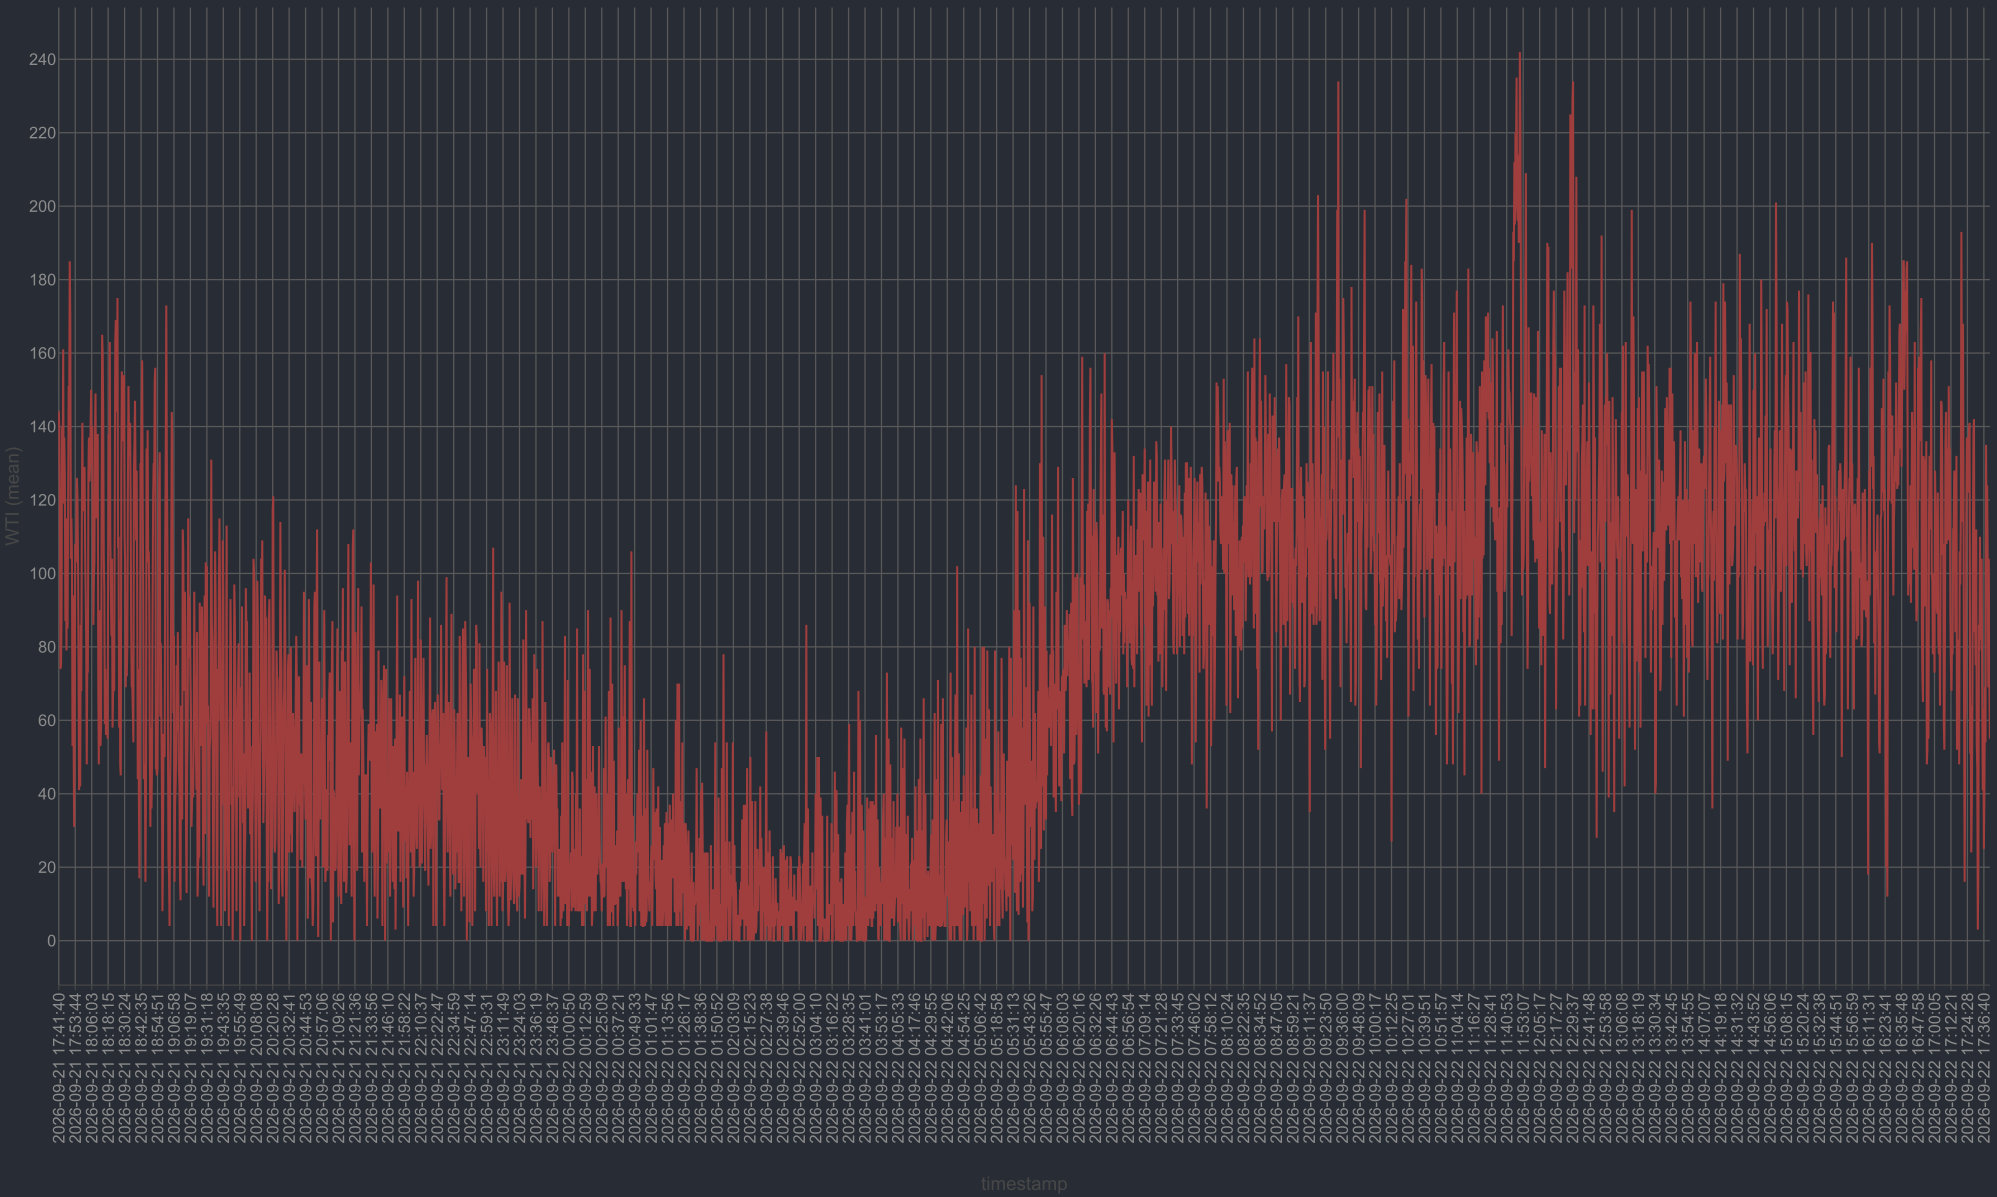
\includegraphics[width=\linewidth]{data/chart1.png}
        \caption{Biểu đồ WTI quan sát của đợt 21--22/09 (\texttt{data/chart1.png}). Vùng đêm có mức thấp, sau đó WTI tăng rõ khi chuyển sang buổi sáng.}
        \label{fig:chart1}
    \end{subfigure}
    \hfill
    \begin{subfigure}[t]{0.48\textwidth}
        \centering
        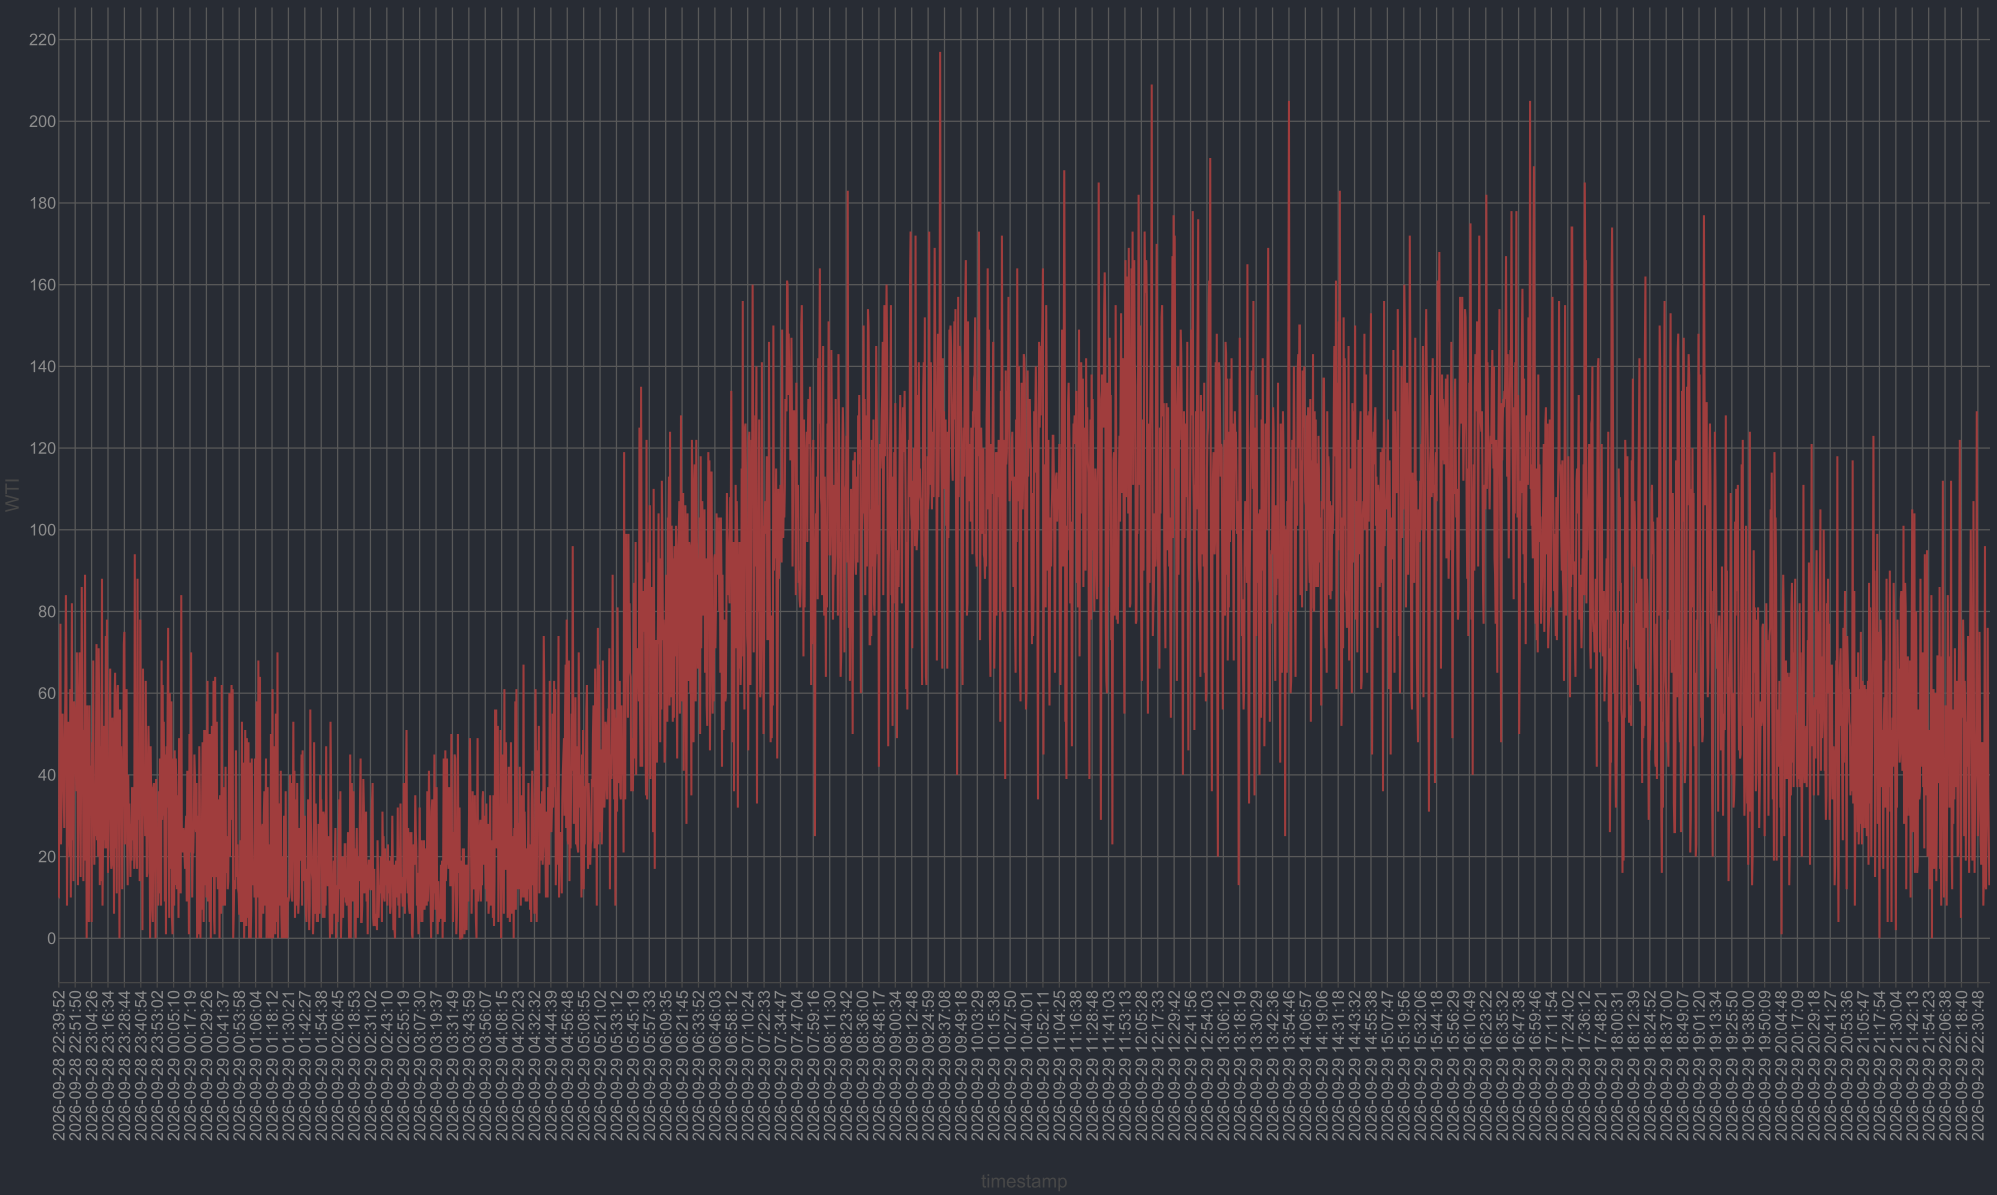
\includegraphics[width=\linewidth]{data/chart2.png}
        \caption{Biểu đồ WTI quan sát của đợt 28--29/09 (\texttt{data/chart2.png}). Hai hình là biểu đồ dữ liệu đã thu, không phải kết quả dự báo.}
        \label{fig:chart2}
    \end{subfigure}
    \caption{Đối chiếu biểu đồ WTI quan sát thực tế giữa hai đợt thu thập dữ liệu.}
    \label{fig:comparison_charts}
    \end{figure}

    Hai đợt đều có WTI trung bình thấp vào khoảng 02 giờ. Tính trên chuỗi phút hoàn tất, giờ có WTI trung bình cao nhất là 11 giờ ở \texttt{data1} và 16 giờ ở \texttt{data2}. Điều này cho thấy vị trí đỉnh và hình dạng chuỗi có thay đổi giữa các đợt; không nên coi một ngày tham chiếu là quy luật cố định. Đỉnh WTI cũng không nhất thiết trùng đỉnh tổng số xe vì thành phần phương tiện có trọng số khác nhau.

    \begin{figure}[htbp]
\centering
\begin{tikzpicture}
    % Định nghĩa 2 màu đặc trưng giống biểu đồ gốc
    \definecolor{colorData1}{RGB}{14, 124, 134} % Xanh teal
    \definecolor{colorData2}{RGB}{217, 119, 36}  % Cam đất

    \begin{axis}[
        title={\textbf{Đối chiếu nhịp ngày của hai đợt thu}},
        title style={font=\normalsize, yshift=2pt},
        width=0.92\textwidth,
        height=6.2cm,
        xlabel={Giờ trong ngày},
        ylabel={WTI trung bình},
        xlabel style={font=\small},
        ylabel style={font=\small},
        tick label style={font=\footnotesize},
        xmin=-0.8, xmax=23.8,
        ymin=7, ymax=138,
        xtick={0,2,4,6,8,10,12,14,16,18,20,22},
        ytick={20,40,60,80,100,120},
        % Cấu hình lưới mờ và trục tọa độ
        grid=both,
        grid style={line width=0.2pt, draw=gray!15},
        axis x line*=bottom,
        axis y line*=left,
        legend style={
            at={(0.97,0.95)},
            anchor=north east,
            draw=gray!30,
            fill=white,
            font=\footnotesize,
            cells={anchor=west}
        }
    ]

        % Đường biểu diễn data1 (Xanh teal)
        \addplot[
            color=colorData1,
            mark=*,
            mark size=1.8pt,
            line width=1.1pt
        ] coordinates {
            (0, 26.5) (1, 16.7) (2, 12.5) (3, 14.8) (4, 19.8) 
            (5, 38.9) (6, 85.0) (7, 99.0) (8, 110.5) (9, 118.2) 
            (10, 114.5) (11, 132.0) (12, 122.3) (13, 109.8) (14, 114.6) 
            (15, 116.8) (16, 115.5) (17, 97.0) (18, 97.5) (19, 60.9) 
            (20, 50.6) (21, 46.7) (22, 43.2) (23, 35.5)
        };
        \addlegendentry{data1}

        % Đường biểu diễn data2 (Cam đất)
        \addplot[
            color=colorData2,
            mark=*,
            mark size=1.8pt,
            line width=1.1pt
        ] coordinates {
            (0, 26.5) (1, 19.0) (2, 16.6) (3, 18.0) (4, 27.2) 
            (5, 52.0) (6, 79.6) (7, 99.5) (8, 106.3) (9, 115.0) 
            (10, 110.4) (11, 109.2) (12, 112.1) (13, 101.5) (14, 106.9) 
            (15, 108.3) (16, 120.0) (17, 99.0) (18, 80.7) (19, 69.6) 
            (20, 53.5) (21, 50.1) (22, 45.6) (23, 34.4)
        };
        \addlegendentry{data2}

    \end{axis}
\end{tikzpicture}
\caption{Đối chiếu biến thiên chỉ số WTI trung bình theo các khung giờ trong ngày giữa data1 và data2.}
\label{fig:hourly_wti_comparison}
\end{figure}
    \subsection{Chất lượng và tính đại diện}
    Kiểm tra trực tiếp cho thấy hai CSV không có ô trống hoặc timestamp trùng. Hàm kiểm tra của dự án chấp nhận toàn bộ bản ghi về số đếm nguyên không âm, giá trị hữu hạn và tính nhất quán của \texttt{total}, WTI. Mã băm SHA-256 của hai CSV hiện tại khớp thông tin dữ liệu trong báo cáo huấn luyện đã lưu.

    Tuy vậy, dữ liệu sạch ở cấp dòng vẫn có thể thiếu theo thời gian: 5 phút hoàn toàn vắng mẫu chỉ xuất hiện rõ sau khi đưa dữ liệu về lưới một phút. Ngoài ra, dữ liệu chưa có \texttt{camera\_id}, phiên bản detector, ROI, nhãn thời tiết, tốc độ hoặc nhãn ùn tắc. Hai đợt gần 24 giờ chưa đủ để đánh giá mùa vụ tuần, ngày lễ, sự cố hay khả năng chuyển sang giao lộ khác.



\section{Quy trình xử lý hệ thống}

    \subsection{Luồng xử lý tổng thể}
    Luồng xử lý dữ liệu được thiết kế khép kín và tự động hóa qua các công đoạn:
    \begin{figure}[htbp]
\centering
\begin{tikzpicture}[
    node distance = 1.2cm and 0.6cm,
    every node/.style = {font=\small},
    block/.style = {
        rectangle, 
        draw=blue!70!black, 
        fill=blue!5, 
        thick,
        rounded corners=3pt,
        align=center, 
        minimum height=1.1cm,
        inner sep=6pt
    },
    line/.style = {
        -Stealth, 
        thick, 
        draw=gray!80
    }
]

    % --- TẦNG 1: XỬ LÝ DỮ LIỆU ĐẦU VÀO ---
    \node [block, text width=2.6cm] (b1) {Ảnh Camera 1};
    \node [block, text width=2.9cm, right=of b1] (b2) {YOLO \& Chia lát ảnh};
    \node [block, text width=2.8cm, right=of b2] (b3) {Đếm phân loại\\\& Tính điểm WTI};
    \node [block, text width=3.0cm, right=of b3] (b4) {Tổng hợp phút\\hoàn tất};

    % --- TẦNG 2: MÔ HÌNH VÀ CẢNH BÁO ---
    \node [block, text width=3.0cm, below=of b4] (b5) {61 đặc trưng};
    \node [block, text width=2.8cm, left=of b5] (b6) {60 bộ hồi quy};
    \node [block, text width=2.9cm, left=of b6] (b7) {Làm mượt};
    \node [block, text width=2.6cm, left=of b7, fill=orange!10, draw=orange!80!black] (b8) {\textbf{Ước tính ETA}\\\textbf{\& Dashboard}};

    % --- CÁC ĐƯỜNG NỐI (MŨI TÊN) ---
    \draw [line] (b1) -- (b2);
    \draw [line] (b2) -- (b3);
    \draw [line] (b3) -- (b4);
    
    % Đường chuyển từ tầng 1 xuống tầng 2
    \draw [line] (b4) -- (b5);
    
    \draw [line] (b5) -- (b6);
    \draw [line] (b6) -- (b7);
    \draw [line] (b7) -- (b8);

\end{tikzpicture}
\caption{Sơ đồ luồng xử lý dữ liệu và suy luận dự báo tổng thể của hệ thống.}
\label{fig:pipeline_flowchart}
\end{figure}

    Song song với luồng xử lý trên, hệ thống lưu quan sát và dự báo đã phát ra vào cơ sở dữ liệu SQLite. Khi dữ liệu tương lai đã đến, script đánh giá có thể đối chiếu dự báo với quan sát đúng thời điểm.

    \begin{table}[htbp]
        \centering
        \caption{Các thành phần chính và trách nhiệm trong hệ thống}
        \vspace{0.2cm}
        \begin{tabular}{|p{4.5cm}|p{11.5cm}|}
            \hline
            \textbf{Thành phần} & \textbf{Trách nhiệm chính} \\
            \hline
            \texttt{core/Get\_frame.py} & Tải và giải mã ảnh từ camera giao thông. \\
            \hline
            \texttt{core/Yolo\_detect.py} & Nhận diện, đếm số lượng phương tiện theo từng lớp và tính WTI. \\
            \hline
            \texttt{core/vision\_worker.py} & Thu ảnh và chạy nhận diện ngoài luồng giao diện người dùng (background thread). \\
            \hline
            \texttt{core/traffic\_features.py} & Kiểm tra tính hợp lệ của mẫu, tổng hợp theo phút, tạo đặc trưng và ma trận mục tiêu. \\
            \hline
            \texttt{training\_model.Py} & Lựa chọn target mode, huấn luyện (fit), đánh giá và lưu trữ model bundle. \\
            \hline
            \texttt{core/traffic\_forecast.py} & Kiểm tra bundle, suy luận dự báo, chạy nhánh dự báo tạm thời và tính ETA. \\
            \hline
            \texttt{core/forecast\_worker.py} & Quản lý lịch sử chuỗi thời gian, hoàn tất phút và cập nhật dữ liệu dự báo. \\
            \hline
            \texttt{core/traffic\_store.py} & Lưu trữ và khôi phục mẫu quan sát, các phiên bản dự báo bằng SQLite. \\
            \hline
            \texttt{ui/traffic\_forecast\_chart.py} & Trực quan hóa chuỗi lịch sử, đường dự báo, đường tham chiếu và ngưỡng cảnh báo. \\
            \hline
        \end{tabular}
    \end{table}

    \subsection{Nhận diện phương tiện và tạo phép đo}
    Hệ thống sử dụng mô hình nhận diện đối tượng \texttt{yolo26x.pt} thông qua thư viện Ultralytics. Để tăng cường khả năng phát hiện phương tiện ở xa và bị che khuất trong khung nhìn rộng của camera, mô-đun tích hợp \texttt{supervision.InferenceSlicer} nhằm chia ảnh thành các lát nhỏ kích thước $256 \times 256$ pixel, thực hiện nhận diện độc lập trên từng lát rồi ghép hợp nhất kết quả. Các class ID COCO được theo dõi gồm: 0 (người), 2 (ô tô), 3 (xe máy), 5 (xe buýt) và 7 (xe tải).

    Chia lát ảnh là một lựa chọn kỹ thuật phù hợp với cảnh camera góc rộng có mật độ phương tiện cao: mỗi lần suy luận chỉ cần xử lý một vùng không gian hẹp với độ phân giải chi tiết. Tuy nhiên, đây là giải thích kỹ thuật về vai trò của kiến trúc, chưa phải kết quả định lượng rằng kỹ thuật chia lát đã cải thiện độ chính xác (Precision/Recall). Dự án hiện tại chưa xây dựng tập ảnh gán nhãn cục bộ kèm phép so sánh có kiểm soát để đo đạc mức độ cải thiện này.

    \begin{figure}[htbp]
        \centering
        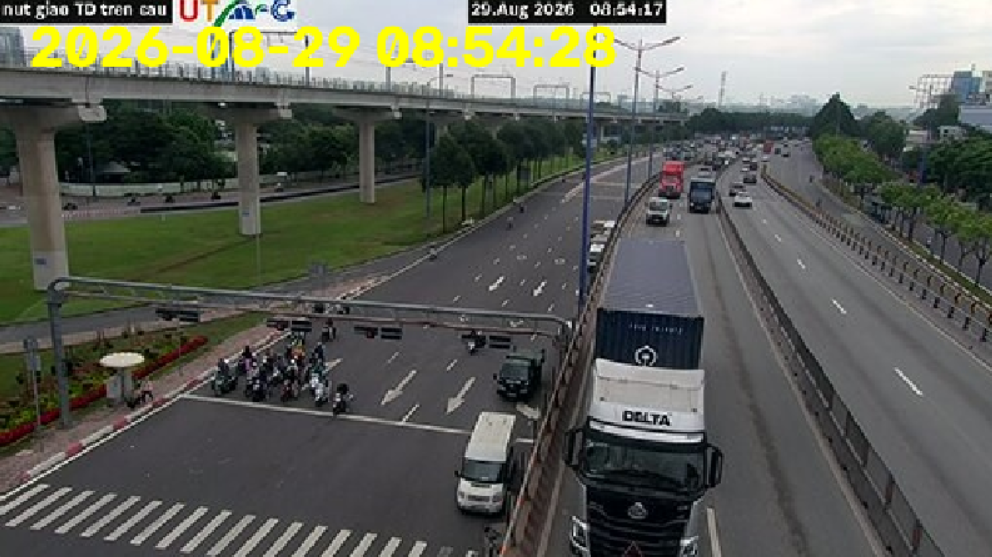
\includegraphics[width=0.85\textwidth]{test_img/1.png}
        \caption{Ảnh thử nghiệm đầu vào \texttt{test\_img/1.png}, ghi nhận các phương tiện ở nhiều khoảng cách và kích thước khác nhau.}
    \end{figure}

    \begin{figure}[htbp]
        \centering
        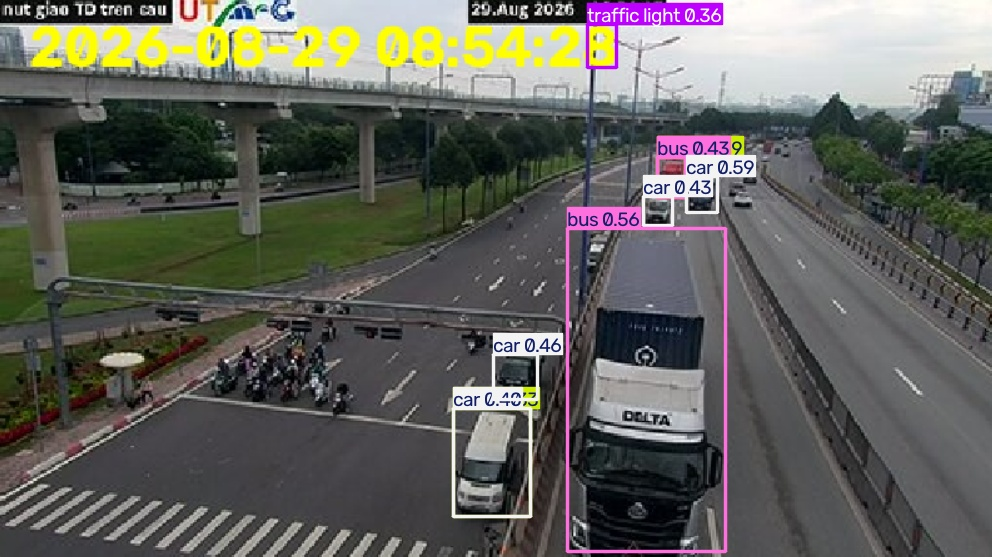
\includegraphics[width=0.85\textwidth]{runs/detect/predict/1.jpg}
        \caption{Kết quả thử nghiệm lưu tại \texttt{runs/detect/predict/1.jpg}. Ảnh hiển thị bounding box, nhãn lớp và độ tin cậy nhận diện.}
    \end{figure}

    Một script thử nghiệm độc lập, \texttt{test\_yolo.py}, khảo sát kích thước lát cắt \texttt{slice\_wh=(512, 512)} và lưu tại \texttt{runs/supervision\_test9.png}. Do đó, không đồng nhất kích thước $512 \times 512$ trong script thử nghiệm với cấu hình lát $256 \times 256$ của luồng vận hành chính thức.

    \subsection{Kiểm tra và tiền xử lý chuỗi thời gian}
    \textbf{Kiểm tra schema:} Pipeline yêu cầu dữ liệu phải có cột \texttt{timestamp} cùng bốn cột đếm phương tiện, \texttt{total} và \texttt{WTI}. \texttt{timestamp} phải hợp lệ, đơn điệu tăng và không trùng lặp; số lượng phương tiện đếm được phải là các số nguyên hữu hạn không âm. Hàm kiểm tra sẽ tính toán lại tổng số xe và chỉ số WTI để phát hiện dữ liệu sai lệch công thức trước khi đưa vào sắp xếp theo thời gian.

    \textbf{Tổng hợp theo phút:} Mỗi khoảng thời gian $[10:00, 10:01)$ được gán mốc nhãn $10:01$, tức thời điểm phút đó đã hoàn tất. Quy ước này giúp ngăn chặn việc sử dụng một phút đang thu thập dở dang như thể đã biết đầy đủ thông tin. Tại mỗi phút hoàn tất, hệ thống tính toán: giá trị trung bình số xe từng loại, trung bình WTI/total, độ lệch chuẩn, giá trị cực đại và số lượng mẫu thu được. Độ lệch chuẩn nội phút sử dụng bậc tự do $\text{ddof} = 0$; những phút chỉ có một mẫu quan sát sẽ có độ lệch chuẩn bằng 0.

    \textbf{Xử lý giá trị thiếu:} Những phút hoàn toàn không thu được mẫu nào được gán giá trị \texttt{NaN} ở các phép đo và số mẫu bằng 0. Pipeline tuyệt đối không tự ý điền giá trị 0 hoặc nội suy để tránh biến khoảng thời gian mất tín hiệu camera thành quan sát giao thông thông thoáng. Hai đầu biên của file CSV không đủ phút sẽ bị loại bỏ. Mọi cửa sổ thời gian bị thiếu lịch sử hoặc thiếu bất kỳ giá trị mục tiêu nào trong 60 phút tiếp theo đều bị loại khỏi tập học có giám sát (supervised dataset).

    \textbf{Chuẩn hóa:} Luồng dự báo không áp dụng các phép biến đổi như \texttt{StandardScaler}, \texttt{MinMaxScaler} hoặc đưa WTI về đoạn $[0, 1]$. Cột \texttt{WTI\_norm} được lưu trong dữ liệu thô theo công thức:
    \[
    \text{WTI\_norm} = \text{WTI} \times [1 + \ln(1 + \text{total})]
    \]
    Mặc dù tên cột chứa tiếp vĩ ngữ ``norm'', công thức này thực chất khuếch đại WTI theo tổng số xe chứ không đưa dữ liệu về khoảng chuẩn. Cả tập đặc trưng lẫn mục tiêu của mô hình hiện tại đều không sử dụng cột này. Việc giữ nguyên WTI ở thang đo gốc giúp sai số MAE và ngưỡng cảnh báo có cùng đơn vị trực quan, dễ đối chiếu.

    \textbf{Chất lượng đầu vào lúc vận hành:} Nhánh mô hình yêu cầu chuỗi 61 phút dữ liệu thực tế liên tục, trong đó mỗi phút phải có ít nhất 3 mẫu hợp lệ. Khi thiếu lịch sử hoặc xuất hiện phút thưa mẫu, hệ thống tự động chuyển sang cơ chế ước lượng tạm thời (nếu có dữ liệu tham chiếu). Khi phút mới nhất hoàn toàn không có mẫu quan sát, hệ thống lập tức dừng đưa ra dự báo.

    \textit{Lưu ý kỹ thuật:} Hàm \texttt{supervised\_data()} trong quá trình huấn luyện và kiểm thử offline chỉ yêu cầu dữ liệu không bị thiếu (\texttt{non-null}), chưa áp dụng đồng loạt điều kiện tối thiểu 3 mẫu/phút như nhánh vận hành thực tế. Vì vậy, tập 956 origin đánh giá offline không đồng nhất hoàn toàn với tập thời điểm mà hệ thống chấp nhận kích hoạt mô hình ngoài thực tế.

    \subsection{Thiết kế 61 đặc trưng}
    Từ chuỗi dữ liệu lịch sử một giờ, hệ thống trích xuất tổng cộng 61 đặc trưng đầu vào cho mô hình:

    \begin{table}[htbp]
        \centering
        \caption{Bảng thiết kế 61 đặc trưng đầu vào}
        \vspace{0.2cm}
        \begin{tabular}{|p{3.2cm}|p{1.5cm}|p{5.5cm}|p{6cm}|}
            \hline
            \textbf{Nhóm đặc trưng} & \textbf{Số lượng} & \textbf{Nội dung chi tiết} & \textbf{Thông tin cung cấp} \\
            \hline
            Phút hiện tại & 11 & Trung bình 4 loại xe; mean, std, max của \texttt{total} và \texttt{WTI}; số mẫu & Mức độ hiện diện, cơ cấu thành phần dòng xe, dao động nội phút và độ phủ dữ liệu. \\
            \hline
            Giá trị trễ (Lags) & 16 & Lag 1, 2, 3, 5, 10, 15, 30, 60 cho cả \texttt{total} và \texttt{WTI} & Nắm bắt trạng thái giao thông gần nhất và mức nền tại các mốc xa hơn trong quá khứ. \\
            \hline
            Thống kê trượt & 26 & Mean (5, 15, 30, 60); std, min, max (5, 15, 30) cho cả \texttt{total} và \texttt{WTI} & Xu hướng trung tâm, biên độ biến thiên và mức độ bất ổn định cục bộ. \\
            \hline
            Độ dốc (Slope) & 6 & Slope 5, 15, 30 cho \texttt{total} và \texttt{WTI} & Hướng tăng/giảm và tốc độ biến thiên trung bình của lưu lượng. \\
            \hline
            Thời gian chu kỳ & 2 & \texttt{hour\_sin}, \texttt{hour\_cos} & Vị trí của thời điểm quan sát trong chu kỳ 24 giờ. \\
            \hline
            \textbf{Tổng cộng} & \textbf{61} & \multicolumn{2}{p{11.5cm}|}{} \\
            \hline
        \end{tabular}
    \end{table}

    Với chuỗi tín hiệu $s$, độ dốc trong mã nguồn được tính bằng công thức hiệu số đơn giản:
    \[
    \text{slope}_w(t) = \frac{s(t) - s(t-w)}{w}
    \]
    Đây không phải là hệ số góc thu được từ phép hồi quy tuyến tính trên toàn bộ cửa sổ $w$. 

    Mã hóa thời gian theo chu kỳ sử dụng hàm $\sin$ và $\cos$:
    \[
    \text{hour\_sin} = \sin\left(\frac{2\pi \times \text{giờ}}{24}\right), \quad \text{hour\_cos} = \cos\left(\frac{2\pi \times \text{giờ}}{24}\right)
    \]
    trong đó giờ là số thực bao gồm cả phần lẻ thập phân tính theo phút. Cách biểu diễn này đảm bảo tính liên tục hình học giữa hai thời điểm ranh giới 23:59 và 00:00.

    Việc khai thác song song cả \texttt{total} và \texttt{WTI} giúp mô hình nắm bắt đồng thời cả mật độ lượng xe lẫn cơ cấu trọng số: hai khung hình có cùng tổng số xe vẫn cho WTI khác biệt rõ rệt khi tỷ lệ xe buýt hoặc xe tải thay đổi. Hàm \texttt{create\_features()} chỉ trích xuất từ dữ liệu hiện tại và quá khứ; hàm \texttt{create\_targets()} dịch chuyển WTI về 60 bước tương lai để tạo nhãn. Cùng một mô-đun được sử dụng đồng bộ cho cả pha huấn luyện lẫn suy luận nhằm loại bỏ rủi ro sai lệch thứ tự cột.

    \subsection{Kiến trúc dự báo và hậu xử lý}
    Hệ thống sử dụng kiến trúc \texttt{MultiOutputRegressor(HistGradientBoostingRegressor)} gồm 60 bộ hồi quy riêng biệt, mỗi bộ phụ trách dự báo cho một bước thời gian (horizon) từ $t+1$ đến $t+60$. Tại thời điểm $t$, tất cả 60 mô hình đều nhận chung vector đầu vào $X(t)$; dự báo tại $t+2$ hoàn toàn không phụ thuộc vào kết quả của $t+1$.

    Thiết kế dự báo trực tiếp (Direct Multi-step) giúp triệt tiêu hoàn toàn hiện tượng tích lũy và khuếch đại sai số qua các bước đệ quy. Ngược lại, do 60 bộ hồi quy học hoàn toàn độc lập, chúng không tự bảo đảm tính liên tục mượt mà của đường cong dự báo theo trục thời gian, đồng thời làm tăng chi phí lưu trữ và suy luận.

    Sau suy luận, chuỗi dự báo được xử lý qua các bước:
    \begin{enumerate}
        \item Chặn dưới giá trị tại 0 ($\max(0, \hat{y})$).
        \item Làm mượt bằng bộ lọc trung bình trượt 3 điểm (Moving Average 3), nối liền với tối đa hai điểm WTI quan sát thực tế gần nhất.
        \item Xác định ETA: Áp dụng quy tắc tìm cửa sổ 5 phút liên tiếp có ít nhất 3 điểm vượt ngưỡng 100 WTI (quy tắc 3/5). Giá trị ETA trỏ đến mốc bắt đầu của cửa sổ đầu tiên thỏa mãn điều kiện.
    \end{enumerate}

    \begin{table}[htbp]
        \centering
        \caption{Các trạng thái hoạt động của hệ thống}
        \vspace{0.2cm}
        \begin{tabular}{|p{4cm}|p{12cm}|}
            \hline
            \textbf{Trạng thái} & \textbf{Ý nghĩa trong hệ thống} \\
            \hline
            \texttt{NORMAL} & Nhánh mô hình không phát hiện cửa sổ vượt ngưỡng nào trong 60 phút tới. \\
            \hline
            \texttt{PROVISIONAL} & Đang hoạt động ở chế độ ước lượng tạm thời và chưa phát hiện nguy cơ vượt ngưỡng. \\
            \hline
            \texttt{WATCH} & Phát hiện cửa sổ dự báo vượt ngưỡng, thời điểm bắt đầu xảy ra sau hơn 5 phút. \\
            \hline
            \texttt{WARNING} & Cửa sổ vượt ngưỡng bắt đầu trong vòng 5 phút tới, hoặc quan sát thực tế đã vượt ổn định. \\
            \hline
            \texttt{INSUFFICIENT\_DATA} & Dữ liệu đầu vào chưa đáp ứng đủ tiêu chuẩn để phát tín hiệu dự báo. \\
            \hline
            \texttt{MODEL\_ERROR} & Xảy ra lỗi trong quá trình suy luận hoặc lỗi cấu trúc dữ liệu bundle. \\
            \hline
        \end{tabular}
    \end{table}

    \subsection{Khởi động và dự báo tạm thời}
    Để giải quyết bài toán khởi động lạnh (Cold-start) khi ứng dụng vừa bật và chưa tích lũy đủ 61 phút quan sát, hệ thống xây dựng một đường tham chiếu gồm 96 ô thời gian (mỗi ô 15 phút) tính từ trung bình của tập \texttt{data1}.

    Hàm \texttt{provisional\_values()} sử dụng tối đa 30 phút thực tế gần nhất để điều chỉnh đường tham chiếu:
    \begin{itemize}
        \item Chênh lệch mức nền giữa thực tế và tham chiếu được dùng để bù trừ mức độ cao/thấp.
        \item Khi có tối thiểu 10 phút dữ liệu thật, hệ thống ước lượng xu hướng biến thiên và chặn hệ số góc trong đoạn $[-1, 1]$ WTI/phút.
        \item Mức độ hiệu chỉnh suy giảm dần theo thời gian qua trọng số hàm mũ $\exp(-h/20)$, và giới hạn độ dốc qua $10 \times [1 - \exp(-h/10)]$, giúp các sai lệch ngắn hạn không bị kéo dài suốt cả giờ.
    \end{itemize}

    Các quan sát tham chiếu được đánh dấu cờ \texttt{is\_reference} và không bao giờ được đưa vào mô hình học máy như dữ liệu thực. Khoảng dữ liệu bị mất trong phiên cũng không bị điền lấp bằng tham chiếu, đảm bảo tính trung thực của phép đo giao thông.



\section{Lựa chọn mô hình và tinh chỉnh siêu tham số}

    \subsection{Cơ sở lựa chọn}

    \subsubsection{Cơ sở lựa chọn kiến trúc thuật toán (Model Selection)}
    Trong bài toán dự báo lưu lượng và tốc độ giao thông đa bước thời gian, mô hình được lựa chọn là HistGradientBoostingRegressor (HGB) được bao bọc bởi kiến trúc MultiOutputRegressor. Sự phối hợp này được thiết lập dựa trên các căn cứ lý thuyết và thực nghiệm sau:
    \begin{itemize}
        \item \textbf{Xử lý mối quan hệ phi tuyến tính phức tạp (Non-linear Correlations):} Dữ liệu giao thông đô thị mang tính chất phi tuyến rõ rệt, bị tác động bởi chu kỳ thời gian, hiệu ứng dòng chảy không gian và các biến cố ngẫu nhiên. HGB — một biến thể ưu việt của thuật toán Gradient Boosted Decision Trees (GBDT) dựa trên phân thùng dữ liệu (binning) — có khả năng xấp xỉ tốt các hàm phi tuyến đa chiều mà không đòi hỏi các giả định nghiêm ngặt về phân phối chuẩn của dữ liệu đầu vào.
        \item \textbf{Kiểm soát độ phức tạp không gian (Spatial Complexity Control):} Thay vì xây dựng một mô hình ma trận giao thông toàn cục có độ phức tạp tính toán tăng theo cấp số nhân, phương pháp tiếp cận hiện tại áp dụng kiến trúc MultiOutputRegressor. Chiến lược này tách biệt việc dự báo chuỗi thời gian nhiều bước (multi-step forecast horizon) thành các bài toán quy nạp song song độc lập cho từng vị trí/cảm biến. Cách tiếp cận này giúp cô lập rủi ro lan truyền lỗi (error propagation) giữa các khu vực không gian khác nhau, đồng thời duy trì chi phí tính toán ở mức tuyến tính đối với số lượng điểm đo.
    \end{itemize}

    \subsubsection{Chiến lược thiết lập không gian siêu tham số (Hyper-parameter Configuration)}
    Chiến lược tối ưu hóa mô hình trong dự án tuân theo các nguyên tắc quản trị thực nghiệm nghiêm ngặt:
    \begin{itemize}
        \item \textbf{Cấu hình tĩnh thay vì Tìm kiếm tự động (Static Configuration vs. Hyper-parameter Search):} Các siêu tham số của mô hình HGB không được khởi tạo thông qua các kỹ thuật quét tự động toàn cục như Grid Search, Random Search hay Bayesian Optimization. Thay vào đó, bộ tham số được ấn định tĩnh dựa trên tri thức chuyên ngành (domain expertise) về bản chất chuỗi thời gian giao thông và các thử nghiệm kiểm chứng cục bộ nhằm tránh hiện tượng quá khớp (overfitting) trên tập kiểm thử.
        \item \textbf{Tập trung xác minh dạng biểu diễn mục tiêu (Target Representation Validation):} Quá trình thực nghiệm tập trung phần lớn năng lực kiểm chứng vào việc lựa chọn dạng biểu diễn của chuỗi giá trị đầu ra:
        \begin{itemize}
            \item \textit{Biểu diễn Tuyệt đối (Absolute Target):} Dự báo trực tiếp giá trị thực tế của biến giao thông tại thời điểm $t + k$.
            \item \textit{Biểu diễn Sai biệt (Delta Target):} Dự báo mức độ biến động $\Delta = Y_{t+k} - Y_t$.
        \end{itemize}
        $\Rightarrow$ \textbf{Kết quả thực nghiệm:} Dạng biểu diễn Absolute Target mang lại độ ổn định cao hơn đáng kể. Biểu diễn Delta tỏ ra nhạy cảm quá mức với nhiễu tần số cao tại thời điểm gốc $t$, dẫn đến hiện tượng tích lũy sai số lớn khi dự báo xa.
    \end{itemize}

    \subsection{Phần thực sự được lựa chọn bằng validation}
    Script thử hai cách đặt mục tiêu, sử dụng cùng cấu hình HGB:

    \begin{table}[htbp]
        \centering
        \caption{So sánh dạng biểu diễn mục tiêu trên tập validation của data1}
        \begin{tabular}{|l|l|c|}
            \hline
            \textbf{Cách biểu diễn} & \textbf{Mục tiêu học} & \textbf{MAE validation sau làm mượt} \\
            \hline
            Absolute & $WTI(t+h)$ & 20,42 WTI \\
            Delta & $WTI(t+h) - WTI(t)$ & 23,79 WTI \\
            \hline
        \end{tabular}
    \end{table}

    Với delta, giá trị hiện tại được cộng trở lại khi suy luận. Trên validation của data1, absolute có MAE thấp hơn nên được chọn. Lựa chọn này chỉ được chứng minh trong cách chia dữ liệu và cấu hình đã thử; không phải kết luận rằng dự báo delta luôn kém hơn.

    Không có \texttt{GridSearchCV}, \texttt{RandomizedSearchCV} hoặc nhật ký tìm kiếm lưới siêu tham số trong luồng train được kiểm tra. Tham số \texttt{--max-iter} cho phép người chạy thay đổi số vòng, nhưng sự tồn tại của tùy chọn không chứng minh đã thử nhiều giá trị và chọn tối ưu.

    \subsection{Cấu hình hiện tại và ý nghĩa của từng tham số}

    \begin{table}[htbp]
        \centering
        \caption{Cấu hình siêu tham số của mô hình HistGradientBoostingRegressor}
        \label{tab:hyperparameter_config}
        \begin{tabular}{|l|c|p{11.5cm}|}
            \hline
            \textbf{Tham số} & \textbf{Giá trị} & \textbf{Vai trò và đánh đổi đối với bài toán} \\
            \hline
            \texttt{max\_iter} & 200 & Số vòng boosting tối đa. Tăng có thể giảm sai số fit nhưng tốn thời gian và dễ bám nhiễu trên các cửa sổ có tương quan cao. \\
            \hline
            \texttt{learning\_rate} & 0,05 & Mức đóng góp của mỗi vòng. Bước nhỏ giúp cập nhật từ từ, nhưng phải xét cùng số vòng; ít vòng với bước quá nhỏ có thể chưa học đủ. \\
            \hline
            \texttt{max\_leaf\_nodes} & 15 & Giới hạn độ phức tạp mỗi cây. Nhiều lá mô tả tương tác chi tiết hơn nhưng dễ ghi nhớ các trạng thái hiếm của chỉ một ngày thu. \\
            \hline
            \texttt{min\_samples\_leaf} & 25 & Yêu cầu đủ mẫu trong lá, hạn chế phân tách dựa trên vài đỉnh nhiễu. Các mẫu chồng lấn vẫn không độc lập, nên 25 mẫu không đồng nghĩa 25 sự kiện khác nhau. \\
            \hline
            \texttt{l2\_regularization} & 5,0 & Hạn chế độ lớn cập nhật ở lá, giúp giảm độ nhạy với nhóm quan sát ít hoặc nhiễu; quá mạnh có thể làm phản ứng với đỉnh thật yếu đi. \\
            \hline
            \texttt{early\_stopping} & False & Không dùng cơ chế validation nội bộ tự động; script tự quản lý validation theo thời gian và khoảng loại trừ mục tiêu. \\
            \hline
            \texttt{random\_state} & 42 & Cố định nguồn ngẫu nhiên có liên quan để hỗ trợ tái lập; không phải tham số nhằm trực tiếp tăng độ chính xác. \\
            \hline
            \texttt{n\_jobs} & 1 & Giới hạn chạy song song ở lớp \texttt{MultiOutputRegressor}. Cùng \texttt{threadpool\_limits(1)}, tránh huy động quá nhiều luồng CPU; chưa có benchmark để khẳng định cấu hình này nhanh nhất. \\
            \hline
        \end{tabular}
    \end{table}

    Các giá trị trên là cấu hình cố định được lưu trong mã, chưa phải ``bộ siêu tham số tối ưu'' có chứng cứ tìm kiếm. Phân tích tác dụng của chúng giải thích lựa chọn kỹ thuật, không thay thế thực nghiệm so sánh các cấu hình.

    Horizon 60 phút, lịch sử 61 điểm, làm mượt 3 phút, ngưỡng 100 WTI và quy tắc 3/5 là các tham số của toàn hệ thống. Chúng tác động đến lượng dữ liệu cần có, độ nhạy cảnh báo và độ trễ, nhưng không nên trộn lẫn với siêu tham số cấu trúc cây. Chưa có bằng chứng ngưỡng 100 đã được chọn theo phân vị 85--90 như trong đề xuất ban đầu.

    \subsection{Chia dữ liệu và ngăn rò rỉ thời gian}
    Quy trình trong \texttt{training\_model.Py} gồm:
    \begin{enumerate}
        \item Tạo 1.098 origin hợp lệ từ data1, mỗi origin có 61 đặc trưng và 60 target.
        \item Lấy phần cuối của chuỗi làm validation, gồm 220 origin. Sau loại các origin có mục tiêu chạm vùng validation, phần fit còn 818 origin; 60 origin sát ranh giới không dùng ở giai đoạn lựa chọn.
        \item Origin fit cuối là 08:20 ngày 22/09; origin validation đầu là 09:21. Target xa nhất của origin fit cuối kết thúc lúc 09:20, trước validation.
        \item So sánh absolute và delta bằng MAE trung bình 60 horizon sau làm mượt, chọn absolute.
        \item Refit trên toàn bộ 1.098 origin data1 rồi đánh giá 956 origin data2. Hai tập phút train/test cách nhau 8.940 phút.
    \end{enumerate}

    Thiết kế không xáo trộn ngẫu nhiên và không lấy dữ liệu tương lai làm feature. Khoảng loại trừ đặc biệt cần thiết vì mỗi origin mang theo cả 60 phút nhãn tương lai: chỉ chia theo timestamp của đầu vào mà bỏ qua phần nhãn sẽ tạo rò rỉ qua ranh giới.

    Validation hiện chỉ bao phủ một phần ngày. Đồng thời data2 đã được phân tích trong nhiều báo cáo của dự án. Nếu tiếp tục sửa phương pháp dựa trên các kết quả này, cần một đợt thu mới giữ riêng để đánh giá cuối; data2 lúc đó không còn là bằng chứng hoàn toàn độc lập cho lựa chọn mới.

    \subsection{Kết quả so sánh đã lưu}
    Bảng \ref{tab:mae_comparison} lấy từ \texttt{models/traffic\_wti\_forecast.metrics.json}. MAE tính theo đơn vị WTI, đối chiếu dự báo đã làm mượt với WTI trung bình phút chưa làm mượt. Báo cáo này kiểm tra dữ liệu và cách tính trong mã, không huấn luyện lại mô hình để tạo bộ điểm mới.

    \begin{table}[htbp]
        \centering
        \caption{So sánh MAE giữa các phương pháp trên tập kiểm thử data2}
        \label{tab:mae_comparison}
        \begin{tabular}{|l|c|c|c|c|c|}
            \hline
            \textbf{Phương pháp} & \textbf{MAE +1} & \textbf{MAE +15} & \textbf{MAE +30} & \textbf{MAE +60} & \textbf{MAE TB 60 horizon} \\
            \hline
            HGB, làm mượt 3 phút & 13,70 & 13,40 & 14,10 & 14,71 & 14,12 \\
            Tham chiếu cùng giờ từ data1 & 14,27 & 14,77 & 14,88 & 14,35 & 14,71 \\
            Giữ nguyên WTI hiện tại & 15,72 & 17,04 & 17,29 & 20,70 & 18,55 \\
            Ngoại suy slope 15 phút & 15,86 & 28,23 & 38,55 & 62,13 & 40,35 \\
            \hline
        \end{tabular}
    \end{table}

    HGB có ưu thế về MAE trung bình, nhưng tại +60 phút, baseline cùng giờ tốt hơn. Ngoại suy tuyến tính có sai số tăng mạnh ở horizon xa: tiếp tục kéo một xu hướng ngắn hạn trong cả giờ là giả định không phù hợp với nhiều đoạn chuỗi đã quan sát.

    \begin{table}[htbp]
        \centering
        \caption{Chỉ số phát hiện vượt ngưỡng trên 956 origin của data2}
        \label{tab:threshold_metrics}
        \begin{tabular}{|l|c|c|}
            \hline
            \textbf{Chỉ số vượt ngưỡng, trên 956 origin} & \textbf{HGB làm mượt 3 phút} & \textbf{Tham chiếu cùng giờ} \\
            \hline
            Origin có tương lai vượt ngưỡng theo quy tắc & 530 & 530 \\
            Cảnh báo đúng & 491 & 500 \\
            Báo nhầm & 7 & 0 \\
            Bỏ sót & 39 & 30 \\
            Precision & 98,59\% & 100,00\% \\
            Recall & 92,64\% & 94,34\% \\
            F1 & 0,9553 & 0,9709 \\
            ETA MAE trên origin cảnh báo đúng & 7,09 phút & 3,95 phút \\
            \hline
        \end{tabular}
    \end{table}

    $F_1 = 0,9553$ không có nghĩa ``dự báo kẹt xe chính xác 95,53\%''. Nhãn ở đây được tạo từ WTI vượt ngưỡng thử nghiệm, đơn vị đánh giá là cửa sổ dự báo chồng lấn, và phép đo chưa có ground truth ùn tắc độc lập.

    ETA MAE chỉ tính trên các origin vừa có sự kiện theo WTI vừa được phương pháp cảnh báo. Những ca bỏ sót không tham gia phép tính ETA. Hai cột ETA cũng dùng tập origin cảnh báo đúng khác nhau; không nên diễn giải chênh lệch như một so sánh ghép cặp tuyệt đối. Báo cáo audit đã lưu có kiểm tra trên tập chung 487 origin, ghi nhận ETA MAE khoảng 7,10 phút cho model và 3,85 phút cho tham chiếu.

    Thử lấy mỗi 60 origin hợp lệ một lần trong báo cáo model chỉ còn 16 origin, trong đó 9 dương tính. MAE trung bình ở tập thưa này là 14,25 WTI, nhưng kích thước nhỏ chưa cho phép kết luận chắc chắn về độ ổn định trên các đợt giao thông độc lập.

    \subsection{Tác động của làm mượt và phiên bản kết quả}

    \begin{table}[htbp]
        \centering
        \caption{Tác động của kỹ thuật làm mượt 3 phút đối với mô hình HGB}
        \begin{tabular}{|l|c|c|}
            \hline
            \textbf{Chỉ số của HGB} & \textbf{Dự báo thô} & \textbf{Dự báo làm mượt 3 phút} \\
            \hline
            MAE trung bình & 14,40 & 14,12 \\
            MAE +1 phút & 12,52 & 13,70 \\
            Báo nhầm & 12 & 7 \\
            Bỏ sót & 32 & 39 \\
            ETA MAE trên các ca cảnh báo đúng tương ứng & 6,26 phút & 7,09 phút \\
            \hline
        \end{tabular}
    \end{table}

    Làm mượt giảm dao động và báo nhầm, nhưng tăng bỏ sót và làm sai số ở phút gần nhất lớn hơn. Chọn một đường cong đẹp hơn trên UI vì thế là quyết định có đánh đổi về chất lượng cảnh báo.

    Trong thư mục còn có \texttt{traffic\_backtest.json}, \texttt{warm\_start\_metrics.json} và báo cáo lịch sử liên quan phiên bản 30 phút. Không sử dụng các kết quả này làm điểm số cho model WTI 60 phút. Các mục \texttt{provisional\_3/5/15/30/60} trong metrics của model có kết quả giống nhau và được audit mô tả là của cách hiệu chỉnh cũ. Mã \texttt{provisional\_values()} hiện đã dùng hiệu chỉnh mức/xu hướng giảm dần; chưa có bộ metric mới tương ứng trong các tệp đã kiểm tra để khẳng định chất lượng của thay đổi này.



\section{Điểm nổi bật và đóng góp của dự án}

    \subsection{Kết nối thị giác máy tính với dự báo chuỗi thời gian}
    Dự án không dừng ở hình có bounding box. Số đếm được chuyển thành một chuỗi đo có timestamp, tổng hợp theo phút, dùng cùng định nghĩa đặc trưng khi train và chạy trực tiếp, rồi biến thành đường dự báo và ETA. Sự liên kết này là đóng góp ứng dụng rõ ràng: mỗi bước có đầu vào và đầu ra có thể kiểm tra, thay vì chỉ trình diễn một mô hình riêng lẻ.

    \begin{figure}[htbp]
        \centering
        % 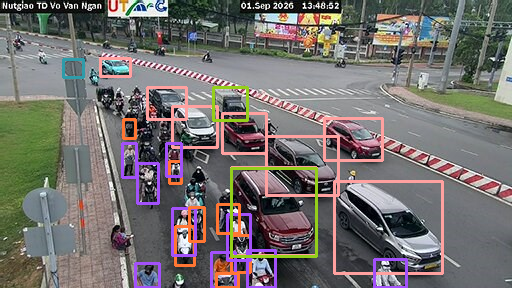
\includegraphics[width=0.85\textwidth]{runs/supervision_test9.png}
        \caption{Kết quả lưu từ thử nghiệm Supervision tại \texttt{runs/supervision\_test9.png}, minh họa nhiều phương tiện nhỏ và che khuất trong cảnh nút giao. Script thử nghiệm sử dụng lát $512 \times 512$; ảnh không phải bảng đo precision/recall và không chứng minh ưu thế định lượng so với lát $256 \times 256$.}
        \label{fig:supervision_test}
    \end{figure}

    \subsection{Phân biệt dữ liệu thật, tham chiếu và dữ liệu mất}
    Khởi động ứng dụng tạo ra một vấn đề thực tế: model cần 61 điểm phút, nhưng người dùng muốn nhìn thấy thông tin ngay. Dự án giải quyết bằng tham chiếu học từ data1, đánh dấu riêng các phút tham chiếu và dùng một nhánh tạm thời. Khi quan sát thật tích lũy, chúng thay thế tham chiếu; khi đủ điều kiện mới chuyển sang model.

    Điểm đáng chú ý là lịch sử tham chiếu không được đưa vào estimator như dữ liệu đo thật, và mất camera sau khởi động không bị che bằng một đường nội suy. Cách xử lý này giữ được ý nghĩa của phép đo và trạng thái chất lượng dữ liệu.

    \subsection{Giữ danh tính nguồn dự báo khi người dùng đổi camera}
    Giao diện cho phép chọn camera để xem, nhưng nguồn dự báo luôn là Camera 1. \texttt{CameraWorker} phát số đếm từ camera dự báo cố định; \texttt{ForecastWorker} loại mẫu có tên camera khác. Nhờ đó thao tác đổi góc xem không làm lịch sử chuỗi thời gian bị trộn giữa hai vị trí.

    Tính độc lập về nguồn không đồng nghĩa độc lập về tài nguyên: việc lấy ảnh và nhận diện camera đang xem thêm vẫn nằm trong vòng worker, có thể làm chu kỳ Camera 1 dài hơn. Chưa có số đo latency để định lượng ảnh hưởng.

    \subsection{Xử lý bất đồng bộ và lưu bằng chứng trước khi biết tương lai}
    Thu ảnh/YOLO và dự báo được đưa ra khỏi luồng giao diện. Model chỉ tải một lần; biểu đồ tái sử dụng Figure và các đối tượng vẽ khi cập nhật. Đây là lựa chọn nhằm giữ UI đáp ứng mà không cần huấn luyện lại hoặc dựng lại toàn bộ biểu đồ mỗi lần có dữ liệu.

    SQLite lưu timestamp quan sát, origin dự báo, thời điểm phát, các giá trị dự báo thô/đã làm mượt, model ID và phương pháp. Script \texttt{evaluate\_live\_forecasts.py} chỉ lấy lần phát đầu tiên của mỗi origin, loại dự báo phát quá muộn và chỉ chấm khi đủ dữ liệu tương lai với độ phủ mẫu yêu cầu. Nhờ vậy việc đánh giá không chọn lại một phiên bản dự báo thuận lợi sau khi đã biết kết quả.

    Lịch sử được khôi phục khi ứng dụng mở lại, nhưng khoảng thời gian ứng dụng tắt vẫn là khoảng thiếu. Collector ghi theo lô ngắn cũng giảm nguy cơ mất toàn bộ đợt thu; việc dừng cưỡng bức vẫn có thể làm mất lô chưa ghi cuối cùng.

    \subsection{Kiểm tra tính tương thích và bảo vệ model đang dùng}
    Bundle dự báo chứa danh sách và thứ tự đặc trưng, horizon, history window, target mode, đường tham chiếu, metrics và thông tin phiên bản môi trường. \texttt{validate\_bundle()} kiểm tra cấu trúc quan trọng trước khi suy luận, bao gồm đủ 60 estimator và đúng thứ tự cột.

    Huấn luyện mới không tự ghi đè artifact đang tồn tại: script chuyển sang tên candidate, lưu model rồi tải lại để so sánh một dự báo với kết quả trước khi lưu. Thiết kế này tạo cơ sở cho việc kiểm tra ứng viên trước khi thay model đang vận hành. Tuy nhiên, script chưa có cổng tự động từ chối triển khai theo toàn bộ tiêu chí cảnh báo; việc lưu thành công không chứng minh model mới tốt hơn.

    \subsection{Kiểm thử hướng vào lỗi có ý nghĩa}
    Các tệp test hiện có bao phủ những tình huống như feature không sử dụng tương lai, đúng thứ tự lag 60, lệch schema, thiếu model, timestamp dự báo, quy tắc 3/5, mất mẫu, phút thưa, đổi camera, khôi phục SQLite, giữ phiên bản forecast và ghi CSV khi có lỗi nhận diện.

    Báo cáo này đọc các kiểm thử để xác định ý đồ và phạm vi bảo vệ của hệ thống, không báo chúng là một lượt test mới đã chạy. Kiểm thử logic hoặc ảnh UI chỉ xác nhận từng phần hành vi; độ chính xác giao thông trực tiếp vẫn cần quan sát tương lai có nhãn và nhật ký tương ứng.

    Những điểm nổi bật trên là đóng góp kỹ thuật trong phạm vi dự án. Tài liệu chưa đưa ra bằng chứng về một thuật toán học máy mới hoặc so sánh học thuật để khẳng định tính mới ở cấp nghiên cứu phương pháp.



\section{Bài học kinh nghiệm}

    \subsection{Định nghĩa đúng đại lượng trước khi tối ưu mô hình}
    WTI tiện cho việc tạo dữ liệu có cấu trúc, nhưng nó là một phép đo thay thế. Nhiều xe trong ảnh có thể vẫn đang di chuyển tốt; một hàng xe ít hơn có thể đang đứng yên. Chỉ tối ưu dự báo WTI không tự giải quyết được khoảng cách giữa ``đông xe trong khung hình'' và ``ùn tắc gây chậm trễ''.

    Bước phát triển tiếp theo nên bắt đầu từ nhãn giao thông độc lập và tiêu chí quan sát rõ ràng, như trạng thái dòng xe hoặc hàng chờ trong một vùng quan tâm. Khi đó mới có cơ sở hiệu chuẩn trọng số, ngưỡng và đánh giá giá trị của cảnh báo. Đây là hướng cải thiện từ giới hạn đã phát hiện, chưa phải chức năng hiện có.

    \subsection{Không có ô trống không có nghĩa chuỗi liên tục}
    Cả hai CSV đều đầy đủ giá trị trên mỗi dòng, nhưng có 5 phút hoàn toàn mất mẫu. Nếu chỉ kiểm tra \texttt{isna()} trên bảng gốc, hệ thống sẽ bỏ qua những khoảng chưa từng được ghi. Chuẩn hóa trục thời gian, giữ NaN và đo số mẫu mỗi phút là cần thiết trước khi tạo lag hoặc kết luận camera đang hoạt động ổn định.

    Chính sách chất lượng cũng cần thống nhất giữa train, backtest và vận hành. Hiện nhánh live yêu cầu tối thiểu 3 mẫu/phút trong lịch sử, còn tập supervised chỉ loại phần thiếu. Đồng bộ tiêu chí này sẽ giúp phép đánh giá phản ánh đúng các thời điểm model thực sự được phép dự báo.

    \subsection{Baseline phải phù hợp với cấu trúc dữ liệu}
    Giữ nguyên giá trị hiện tại là một đối chứng dễ hiểu, nhưng chưa đủ khi chuỗi có biến động theo giờ. Baseline cùng giờ từ data1 đạt MAE rất gần HGB và tốt hơn ở F1 cùng ETA trong lần đánh giá đã lưu. Vì vậy ``thắng persistence'' chưa đủ để khẳng định phần học máy mang lại lợi ích rõ rệt cho mục tiêu cảnh báo sớm.

    Các lần đánh giá sau nên tiếp tục giữ baseline theo giờ, đồng thời kiểm tra trên nhiều đợt mới. Chưa nên biến kết quả một capture thành kết luận HGB hoặc baseline sẽ luôn vượt trội.

    \subsection{Đường dự báo đẹp và cảnh báo hữu ích là hai mục tiêu khác nhau}
    Làm mượt giảm MAE trung bình và báo nhầm, nhưng tăng bỏ sót từ 32 lên 39 origin. Điều này cho thấy tham số hiển thị có thể thay đổi hành vi cảnh báo. Khi thiết kế tiếp, cần xác định trước chi phí bỏ sót, mức báo nhầm chấp nhận được và thời gian cảnh báo hữu ích; không chỉ chọn cấu hình theo một MAE trung bình.

    ETA MAE cũng cần được báo cùng recall và số ca không có ETA. Một phương pháp chỉ cảnh báo các ca dễ có thể có ETA đẹp nhưng bỏ qua nhiều tình huống cần quan tâm.

    \subsection{Bảo toàn thứ tự thời gian cả trong học và chấm điểm}
    Khoảng loại trừ 60 phút ở ranh giới validation là bài học có thể tái sử dụng cho dự báo đa bước: ranh giới phải xét toàn bộ vùng target. Tương tự, nhật ký dự báo phải được lưu trước khi dữ liệu tương lai đến, và phép chấm không được chọn các bản sửa muộn để làm kết quả tốt hơn.

    Các cửa sổ chồng lấn giúp tăng số mẫu huấn luyện nhưng không tăng tương ứng số tình huống độc lập. Báo cáo chất lượng nên bổ sung đánh giá theo đợt sự kiện, ngày thu và thời điểm khởi phát; đồng thời công bố tỷ lệ thời gian hệ thống phải tạm ngừng vì dữ liệu không đủ.

    \subsection{Quản lý phiên bản là một phần của độ tin cậy}
    Thư mục dự án lưu cả đề xuất ban đầu, báo cáo total 30 phút, bản chuyển sang WTI 60 phút, audit và các sửa đổi vận hành. Đọc một báo cáo cũ mà không đối chiếu code có thể dẫn đến mô tả sai target, ngưỡng, thời điểm ghi timestamp, cách dự báo tạm thời hoặc khả năng lưu dữ liệu.

    Mỗi kết quả về sau nên gắn với mã nguồn, dữ liệu, model, cấu hình và môi trường cụ thể. Metadata hiện có đã là nền tảng tốt; cần tiếp tục đảm bảo mọi thay đổi ở logic tạm thời hoặc điều kiện đầu vào đều có đánh giá tương ứng, thay vì dùng lại điểm số của phiên bản trước.

    \subsection{Ưu tiên cho vòng phát triển tiếp theo}

    \begin{table}[htbp]
        \centering
        \caption{Các ưu tiên và tiêu chí hoàn thành cho vòng phát triển tiếp theo}
        \label{tab:future_priorities}
        \begin{tabular}{|c|p{7.5cm}|p{7.5cm}|}
            \hline
            \textbf{Ưu tiên} & \textbf{Việc cần làm} & \textbf{Bằng chứng hoàn thành cần có} \\
            \hline
            1 & Thu thêm nhiều ngày và lưu camera ID, phiên bản detector, cấu hình vùng quan tâm & Dữ liệu có nguồn gốc rõ ràng, bao phủ các thời đoạn và điều kiện quan sát khác nhau \\
            \hline
            2 & Gán nhãn một tập ảnh và trạng thái giao thông độc lập & Sai số đếm/phân loại theo lớp, điều kiện ảnh và đánh giá ngưỡng với nhãn thực \\
            \hline
            3 & Đồng nhất tiêu chí số mẫu giữa train, replay và live & Backtest phản ánh đúng điều kiện được phép dự báo, kèm tỷ lệ bao phủ \\
            \hline
            4 & Chấm lại nhánh tạm thời đang dùng trên dữ liệu mới & So sánh cùng origin giữa tham chiếu thuần, hiệu chỉnh mức/xu hướng và nhánh model \\
            \hline
            5 & Đánh giá cảnh báo theo sự kiện và thời điểm khởi phát & Báo nhầm/giờ, bỏ sót đợt, lead time, ETA trên tập chung và các trường hợp không cảnh báo \\
            \hline
            6 & Đo khả năng vận hành trên máy triển khai & Độ trễ, bộ nhớ, ảnh hưởng khi đổi camera và tỷ lệ thời gian đủ dữ liệu \\
            \hline
        \end{tabular}
    \end{table}

    Hệ thống đã tạo được nền tảng để kiểm tra những câu hỏi này bằng dữ liệu: có quy trình thu, feature dùng chung, baseline, model đa bước và nhật ký dự báo. Giá trị của vòng phát triển tiếp theo nằm ở việc bổ sung bằng chứng về phép đo và hiệu quả cảnh báo, trước khi tăng độ phức tạp của mô hình.

%  Chuyển phần mã nguồn xuống dưới cùng thành Phụ lục (Appendix) 
\newpage
\appendix
\section{Mã nguồn (Source Codes)}
\subsection{Các thư viện được sử dụng}
\begin{minted}[linenos, breaklines, frame=lines, fontsize=\small]{python}
import requests
import cv2
import numpy as np
import time
    
\end{minted}
\subsection{Get\_frame.py}
\begin{minted}[linenos, breaklines, frame=lines, fontsize=\small]{python}
def get_traffic_image(name="Camera 1"):
    global cam_id
    timestamp = int(time.time() * 1000)
    url = f"https://giaothong.hochiminhcity.gov.vn/render/ImageHandler.ashx?id={cam_id[name]}&t={timestamp}"

    headers = {
        "User-Agent": "Mozilla/5.0 (Windows NT 10.0; Win64; x64) AppleWebKit/537.36",
        "Referer": "https://giaothong.hochiminhcity.gov.vn/Map.aspx"
    }

    try:
        response = requests.get(url, headers=headers, timeout=5)
        if response.status_code == 200:
            img_array = np.asarray(bytearray(response.content), dtype=np.uint8)
            frame = cv2.imdecode(img_array, cv2.IMREAD_COLOR)
            return frame
        else:
            print(f"Server response error: {response.status_code}")
    except requests.exceptions.RequestException as e:
        print(f"Network error: {e}")

    return None
\end{minted}

\subsection{Yolo\_detect.py}
\begin{minted}[linenos, breaklines, frame=lines, fontsize=\small]{python}
def callback(image_slice: np.ndarray) -> sv.Detections:
    result = model(image_slice)[0]
    return sv.Detections.from_ultralytics(result)

def image_processing(frame):
    slicer = sv.InferenceSlicer(callback=callback, slice_wh=(256, 256))
    detections = slicer(frame)

    # Đếm theo class ID của YOLO
    class_ids = detections.class_id

    person_count = np.sum(class_ids == 0)
    car_count = np.sum(class_ids == 2)
    motorbike_count = np.sum(class_ids == 3)
    bus_count = np.sum(class_ids == 5)
    truck_count = np.sum(class_ids == 7)
    total_vehicles = car_count + motorbike_count + bus_count + truck_count
    total_objects = len(class_ids)

    print(f"Person: {person_count}")
    print(f"Car: {car_count}")
    print(f"Motorbike: {motorbike_count}")
    print(f"Bus: {bus_count}")
    print(f"Truck: {truck_count}")
    print(f"Total vehicles: {total_vehicles}")
    print(f"Total objects detected: {total_objects}")

    # Weighted Traffic Impact (WTI)
    car_w = 4
    motorbike_w = 1
    bus_w = 7
    truck_w = 6

    weighted_traffic_impact = (
            int(car_count) * car_w
            + int(motorbike_count) * motorbike_w
            + int(bus_count) * bus_w
            + int(truck_count) * truck_w
    )

    weighted_traffic_impact_norm = (
        weighted_traffic_impact / total_vehicles if total_vehicles > 0 else 0.0
    )

    box_annotator = sv.BoxAnnotator(thickness=1)

    annotated_frame = box_annotator.annotate(
        scene=frame.copy(),
        detections=detections
    )

    current_time = datetime.now().strftime("%Y-%m-%d %H:%M:%S")
    cv2.putText(annotated_frame, f"{current_time}", (15, 35),
                cv2.FONT_HERSHEY_SIMPLEX, 1, (0, 255, 255), 2)

    return annotated_frame, person_count, car_count, motorbike_count, bus_count, truck_count, total_vehicles, weighted_traffic_impact, weighted_traffic_impact_norm
\end{minted}

\end{document}